
% this file is called up by thesis.tex
% content in this file will be fed into the main document

%: ----------------------- introduction file header -----------------------


%\begin{savequote}[50mm]
%The beginning is the most important part of the work.
%\qauthor{Plato}
%\end{savequote}




\chapter{Preliminares}
\label{cha:Introduction}

% the code below specifies where the figures are stored
%\ifpdf
   % \graphicspath{{1_introduction/figures/PNG/}{1_introduction/figures/PDF/}{1_introduction/figures/}}
%\else
 %   \graphicspath{{1_introduction/figures/EPS/}{1_introduction/figures/}}
%\fi


%-------------------------------------------------------------------------

%\cite{turing1950computing}




% ----------------------------------------------------------------------

\section{La ecuaci\'on diferencial hipergeom\'etrica y sus soluciones  } \label{sec:sol_ec_hip}

Consideremos la siguiente serie :

$$F(a,b,c;x)= \sum_{n=0}^{\infty } \frac{(a)_{n} (b)_{n}}{(c)_{n}(1)_{n}} x^{n}$$

En donde $x$ es una variable compleja , $(\alpha)_{n} = \alpha (\alpha +1)(\alpha +2)\cdots (\alpha +n-1)$, %cuando n= 0? %

y $c \neq 0, -1, -2,...$. Esta serie es la llamada serie hipergeométrica.  El coeficiente $n$-\'esimo de esta serie al que llamaremos $A_{n}$ esta dado por $$A_{n}=\frac{a(a+1)\cdots (a+n-1) \cdot b(b+1)\cdots(b +n -1) }{c(c+1)\cdots (c+n-1) \cdot 1 (1+1) \cdots (n)}$$ De esta igualdad obtenemos:

\begin{equation}
\frac{A_{n+1}}{A_{n}}= \frac{(a+n)(b+n)}{(c+n)(1+n)}
\end{equation}

Usando el criterio del cociente podemos notar que el radio de convergencia de esta serie es 1, cuando $a$ o $b$ son negativos  la serie es finita. De cualquier modo tenemos que dicha serie define una funci\'on holomorfa en $x$ en al menos el disco de radio 1 centrado en 0 y tambi\'en es holomorfa en $(a,b,c)$ si $c \neq 0, -1, -2,...$ \\

Nuestro inter\'es por la serie definida anteriormente viene del hecho que dicha serie es una soluci\'on de la ecuaci\'on diferencial hipergeom\'etrica

$$ x(1-x)\frac{d^{2}u}{dx^{2}} + \lbrace c- (a+b+1)x \rbrace \frac{du}{dx} -abu=0 $$

 A la cual denotamos $E(a,b,c;x)$ y la referimos como la serie hipergeom\'etrica con par\'ametros $(a,b,c)$. Para ver que $F(a,b,c;x)$ es una soluci\'on de $E(a,b,c)$ procedemos como Euler e introducimos el operador $ D = x \frac{d}{dx}$, a continuaci\'on  enunciamos algunas  propiedades que son \'utiles:


\begin{enumerate}
\item $Dx^{n}= nx^{n}$
\item $f(D)x^{n}=f(n)x^{n}$ donde $f$ es un polinomio de coeficientes constantes
\end{enumerate}

La propiedad n\'umero 1 es clara de la definici\'on, para la propiedad n\'umero 2 debemos dejar en claro como funciona el operador $D^{n}$ al aplicarlo a $x^{n}$. Cuando $n=2$ tenemos que $D^{2} x^{n} = x\frac{d}{dx} (x\frac{d}{dx} (x^{n}) )= x\frac{d}{dx}(x \cdot nx^{n-1})=x\frac{d}{dx} (nx^{n} ) = x\cdot n^{2}x^{n-1}=n^{2}x^{n}$, en general se tiene por un proceso an\'alogo al anterior que $D^{m}x^{n}=n^{m}x^{n}$.Sea

$$ f(x)= \sum_{i=0}^{n} a_{i}x^{i} $$

Donde $a_{n} \neq 0$, un polinomio de grado n y por $f(D)$ entendemos el operador $$f(D) = \sum_{i=0}^{n} a_{i}D^{i}$$

Entendiendo $D^{i}$ como la composici\'on del operador $D$ $i$-veces consigo mismo. Aplicamos este operador a $x^{n}$ y obtenemos

$$f(D)x^{n}=(\sum_{i=0}^{n}a_{i}D^{i}) x^{n} = \sum_{i=0}^{n}a_{i} D^{i}( x^{n}) = \sum_{i=0}^{n}a_{i}n^{i}x^{n} = f(n)x^{n}   $$


Gracias a este operador $D$ podemos escribir la ecuaci\'on diferencial hipergeom\'etrica en t\'erminos de dicho operador para obtener;

$$E(a,b,c): [(a+D)(b+D)- (c+D)(1+D)\frac{1}{x}]u=0$$

Con esta nueva presentaci\'on verificamos que la serie $F(a,b,c;x)$ es una soluci\'on de dicha ecuaci\'on. \\

Podemos escribir

$$F(a,b,c;x)= \sum_{n=0}^{\infty } \frac{(a)_{n} (b)_{n}}{(c)_{n}(1)_{n}} x^{n} = \sum A_{n} x^{n}$$

Y evaluamos

$$[(a+D)(b+D)- (c+D)(1+D)\frac{1}{x}] \sum A_{n}x^{n}$$
$$= \sum [(a+D)(b+D)A_{n}x^{n}- (c+D)(1+D)A_{n}x^{n-1}]$$
$$= \sum [(a+n)(b+n)A_{n}x^{n}- (c+n-1)(1+n-1)A_{n}x^{n-1}]$$
$$= \sum [(a+n)(b+n)A_{n}x^{n}- (c+n)(1+n)A_{n}x^{n}]=0$$


La \'ultima igualdad se da gracias a que obtenemos una serie telesc\'opica. Esta serie tiene singularidades en $0,1$ e $\infty$, nuestro objetivo ahora es encontrar soluciones en los puntos singulares como hicimos anteriormente con $x=0$. Denotaremos  a la soluci\'on  $F(a,b,c;x)$ como $f_{0}(x;0)$. \\

Queremos hallar otra soluci\'on en $x=0$ pero para esto necesitamos calcular la aplicaci\'on del operador $D$ al t\'ermino $x^{s} u$;

$$D(x^{s}u)= sx^{s}u + x^{s}Du = x^{s}(s +D)u$$

esto es $Dx^{s}= x^{s} (s + D)$, con este c\'alculo podemos obtener una expresi\'on equivalente para

$$[(a+D)(b+D) - (c+d)(1+d) \frac{1}{x}] x^{1-c} $$

La expresi\'on anterior es equivalente a

$$x^{1-c}[(a+1-c+D)(b+1-c+D)-(1+D)(2-c+D)\frac{1}{x}]$$

y esto nos dice que

$$x^{1-c} F(a+1-c,b+1-c,2-c:x) $$

Es tambi\'en una soluci\'on de $E(a,b,c)$. Aunque la serie anterior esta definida solamente cuando $2-c$ no es un entero negativo o cero (cuando es $c=1$ la serie  coincide con $F(a,b,c;x)$) esto no afecta nuestra soluci\'on ya que tomamos $1-c \in i\mathbb{R}$ en cuyo caso siempre esta definida. A esta ultima soluci\'on la denotamos por $f_{0}(x;1-c)$.

Queremos hallar tambi\'en soluciones alrededor del punto singular $x=1$, llevamos a cabo una transformaci\'on de la variable $x$ en $1-x$ abusando de la notaci\'on, y verificamos como luce ahora

$$E(a,b,c)=x(1-x) \frac{d^{2}u}{dx^{2}} + \lbrace c- (a+b+1)x \rbrace \frac{du}{dx} -abu$$

 Bajo esta transformaci\'on el primero y el tercer t\'ermino no cambian, pero el segundo t\'ermino ahora es

$$-\lbrace  c- (a+b+1)(1-x)\rbrace = a+b+1-c-(a+b+1)x $$

Entonces podemos notar que la ecuaci\'on transformada es de nuevo la ecuaci\'on hipergeom\'etrica con par\'ametros $ (a,b,a+b+1-c)$ y a menos que $c-a-b$ sea entero obtenemos como antes dos soluciones pero ahora alrededor de $x=1$

$$F(a,b,a+b+1-c;1-x), \ \ (1-x)^{c-a-b}F(c-a,c-b,c+1-a-b;1-x)$$

En nuestro caso tomamos $c-a-b \in i\mathbb{R} $ por lo que las soluciones anteriores siempre estan definidas en su radio de convergencia. A las soluciones anteriores las denotamos $f_{1}(x;0) $ y $f_{1}(x;c-a-b)$ respectivamente.

\section{Continuaci\'on anal\'itica}

La continuaci\'on anal\'itica nos da una forma de extender el dominio sobre el cual una funci\'on anal\'itica esta definida, si tomamos la serie de potencias,

\begin{equation} \label{serie de potencias}
 f(z) = \sum_{k=0}^{\infty} a_{k} (z-z_{0})^{k}
\end{equation}


Esta serie de potencias generalmente es v\'alida en un radio de convergencia dado, en ciertos casos $f$ tiene una serie de potencias que es v\'alida mas all\'a del radio de convergencia esperado, y esta serie de potencias puede servir para definir la funci\'on $f$ fuera de su dominio de definici\'on original.

Sean $f_{1},f_{2}$ funciones anal\'iticas en dominios $\Lambda_{1},\Lambda_{2}$ respectivamente, supongamos adem\'as que la intersecci\'on $\Lambda_{1} \cap \Lambda_{2}$ es no vac\'ia y $f_{1}=f_{2}$ en $\Lambda_{1} \cap \Lambda_{2}$, en este caso llamamos a $f_{2}$ la continuaci\'on anal\'itica de $f_{1}$ a $\Lambda_{2}$ y viceversa, A\'un m\'as si dicha extensi\'on existe es \'unica.

Para dar una definici\'on formal supongamos que $f$ es anal\'itica en una vecindad $U_{z_{0}}$ de $z_{0}$ y $\gamma: [a,b] \rightarrow D $ un camino en $D$ basado en $z_{0}$.


\begin{defn}
Sea $f^{*}:[a,b] \rightarrow \mathbb{C}$  una funci\'on continua con las siguientes propiedades:
\begin{enumerate}
\item $f^{*}(t) =f (\gamma (t))$  para $t$ cercano a $a$ (en $[a,b]$).
\item Para cada $t' \in [a,b]$, hay una funci\'on $h_{t'}(z)$ anal\'itica en un disco $D_{t'}$ sobre $\gamma (t')$ con $h_{t'}(\gamma (t)) = f^{*}(t)$ para $t$ cercano a $t'$ en $[a,b]$
\end{enumerate}
Si tal $f^{*}$ existe esto nos define $h_{t'}(z)$. Esta es la continuaci\'on anal\'itica de $f$ a $t'$. Es una funci\'on anal\'itica en alguna vecindad de $\gamma (t')$. Nos interesa realmente la funci\'on $h_{b}(z)$ anal\'itica en una vecindad de $\gamma (b)$. Le llamamos $f_{\gamma} (z) = f_{\gamma}$, la continuaci\'on anal\'itica de $f$ (a lo largo de $\gamma$).
\end{defn}

Nuestro inter\'es en la continuaci\'on anal\'itica radica en la manera de hallar el grupo de monodrom\'ia, si tenemos un punto $a \in \mathbb{C}$ y una vecindad $U_{a}$ en la cual tenemos un conjunto de soluciones linealmente independientes, la monodrom\'ia que mas adelante analizamos con m\'as detalle tiene relaci\'on con la continuaci\'on anal\'itica de las soluciones de una ecuaci\'on diferencial a traves de lazos anclados en $a$ y sus clases (es decir el grupo fundamental) y las matrices que relacionan a estas soluciones.

Cuando tratamos con la ecuaci\'on hipergeom\'etrica, el teorema fundamental de Cauchy nos dice que para cada punto $x_{0} \neq 0,1$ existen dos soluciones holomorfas linealmente independientes alrededor de $x_{0}$, en otras palabras, el conjunto de estas soluciones forman un espacio lineal bidimensional sobre $\mathbb{C}$. Cualquiera de estas soluciones se puede continuar anal\'iticamente a lo largo de cualquier lazo en $\mathbb{C} - \lbrace0,1 \rbrace$. Las soluciones en general no son univaluadas. Si $\gamma$ es un lazo anclado en $x_{0}$ y $u_{1}$ una soluci\'on no cero, y $u_{2}$ otra soluci\'on que no es m\'ultiplo constante de $u_{1}$ y sean $\gamma^{*} u_{1}$ y $\gamma^{*} u_{2}$ las continuaciones anal\'iticas a trav\'es de $\gamma$, como $\gamma^{*} u_{1},\gamma^{*} u_{2}$ siguen siendo soluciones linealmente independientes se tiene que existe una matriz $M(\gamma) \in GL(2,\mathbb{C})$ que relaciona a estas soluciones, esta matriz se llama la matriz de conexi\'on de $(u_{1},u_{2})$ a lo largo de $\gamma$.

\begin{figure}[h]
  \centering
  % Requires \usepackage{graphicx}
  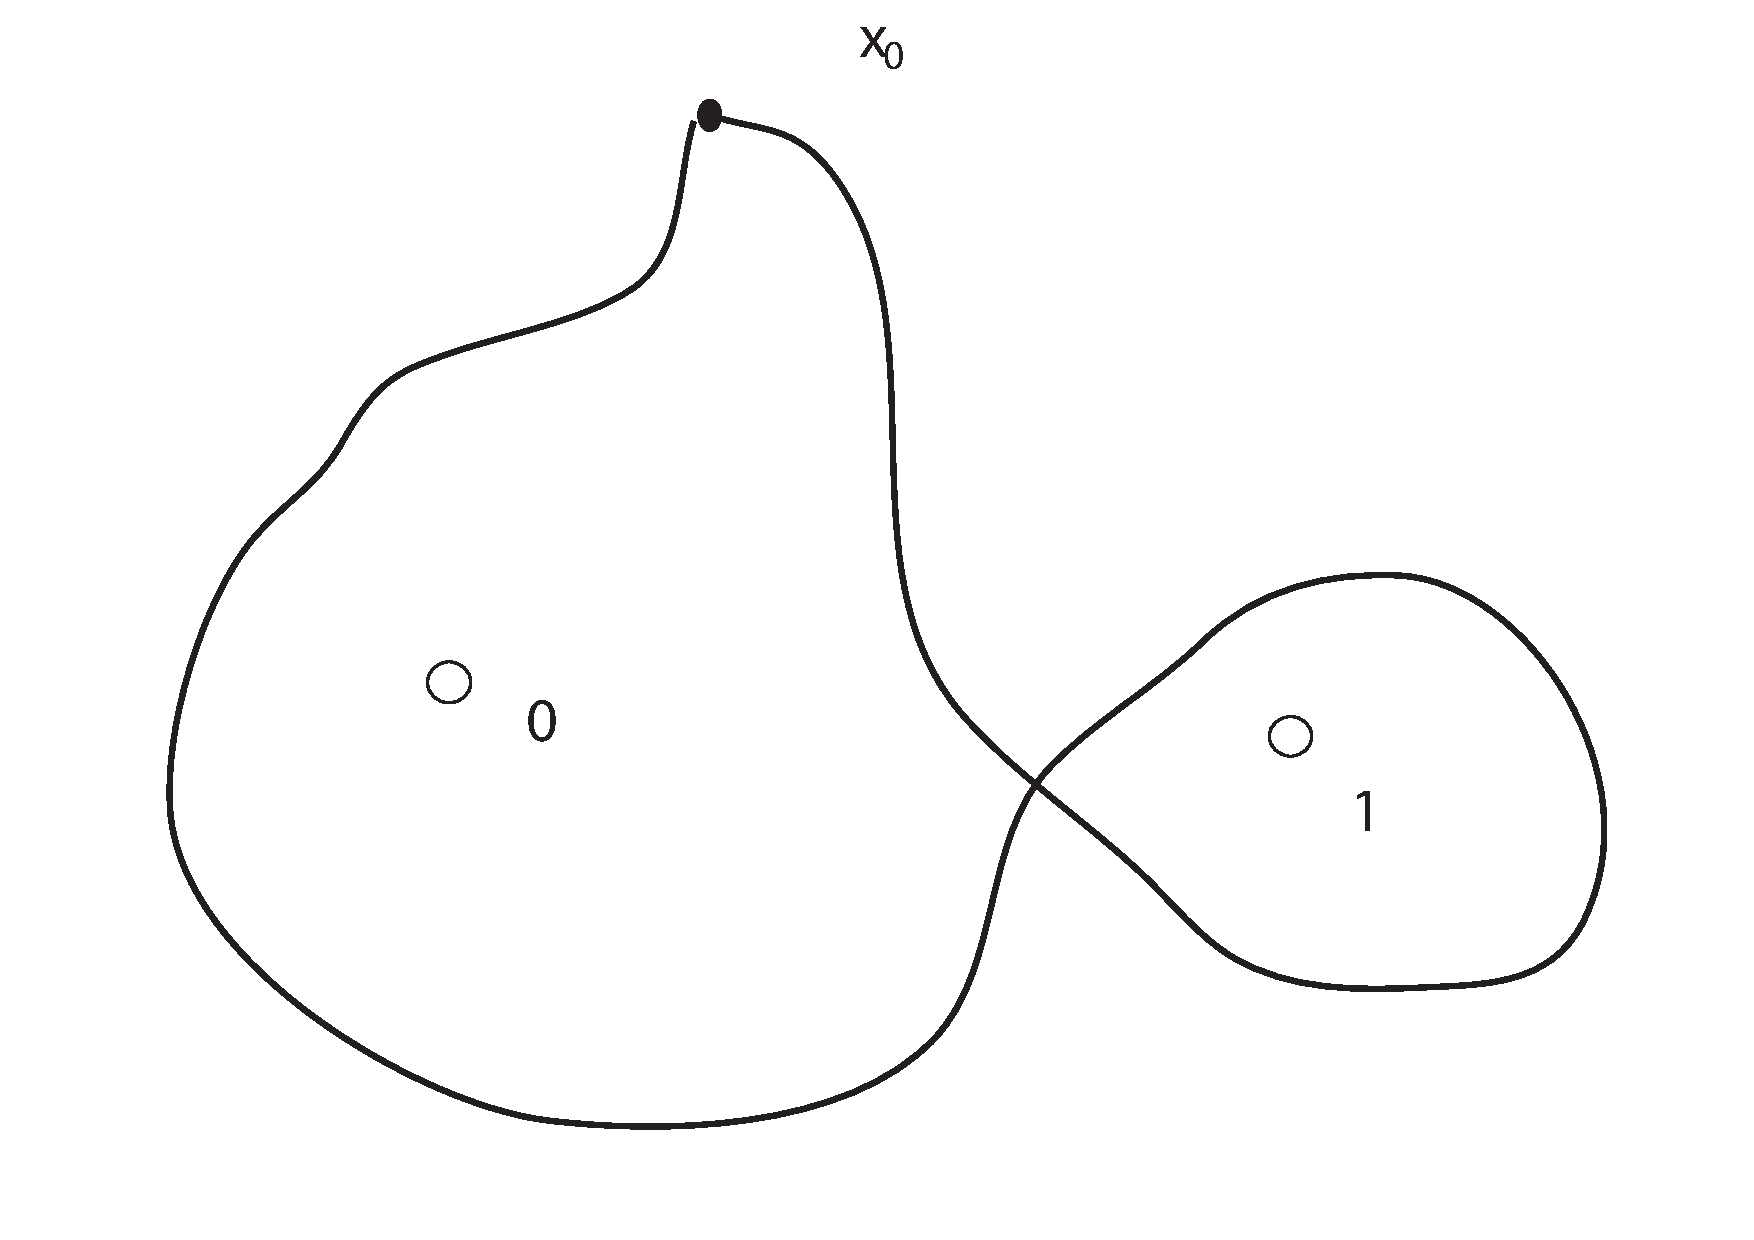
\includegraphics[width=8cm]{continuacion-analitica.pdf}\\
  \caption{Lazo anclado en un punto en $\mathbb{C}- \lbrace 0,1 \rbrace$ }\label{continuacion-analitica}
\end{figure}


Las matrices de conexi\'on juegan un papel fundamental en nuestra b\'usqueda del grupo de monodrom\'ia.

\section{Grupos Klenianos y grupos de Schotkky}

De entre los ejemplos de subgrupos discretos de isometr\'ias hiperb\'olicas conocidos, los grupos de Schotkky son ejemplos cl\'asicos de estos, al ser nuestro objetivo dar un ejemplo de un grupo de Schotkky tenemos la obligaci\'on de dar una definici\'on e introducir brevemente algunos resultados interesantes.

\begin{defn}
Un grupo de Schotkky  es un grupo generado por transformaciones de Möbius $g_{1},..g_{k},k \geq 1$ junto con una colecci\'on de pares de regiones disjuntas en $\widehat{\mathbb{C}}$, digamos $C_{1},B_{1},..,C_{k},B_{k}$, acotadas por curvas de jordan,tal que $g_{i} (C_{i}) = \widehat{\mathbb{C}} - \bar{B_{i}}$ para toda $i=1,..k.$, el conjunto $g_{1},..,g_{k}$ es llamado un conjunto de generadores Schotkky, los dominios $C_{i},B_{i}$ un conjunto fundamental de dominios y el entero $k$ el g\'enero del grupo de Schottky.
\end{defn}

Todos los grupos de Schottky son grupos finitamente generados tal que todos sus elementos no triviales son loxodr\'omicos, cuando decimos elementos no triviales nos referimos a todos excepto la identidad.

Un grupo de Schottky es cl\'asico si las curvas de jordan correspondientes a alg\'un conjunto de generadores se pueden escoger como c\'irculos.

Un grupo de Schottky tambi\'en puede ser caracterizado de la siguiente manera

\begin{thm}
Un grupo $G < PSL(2,\mathbb{C})$ es un grupo de Schottky si y solo si $G$ es finitamente generado, y un grupo Kleniano puramente loxodr\'omico que es isomorfo a un grupo libre.
\end{thm}

En nuestro caso la noci\'on de grupo de Schottky que usamos es la siguiente: Consideremos una familia de pares de 2-discos disjuntos $D_{1},..,D_{s}$ en la 2-esfera cuyas fronteras son los c\'irculos $C_{1},..,C_{s}$ y sean $\gamma_{1},..,\gamma_{s}$ inversiones en estos $s$ c\'irculos y sea $G$ el grupo generado por estas inversiones. Le llamamos a $G$ un grupo de Schottky. El subgrupo de \'indice 2 de longitud par es un grupo de Schottky cl\'asico.

El t\'ermino grupo Kleniano se utiliza para referirse a cualquier subgrupo discreto de isometr\'ias hyperb\'olicas siendo cierto o no que su regi\'on de discontinuidad sea vac\'ia.

Si el lector desea conocer todos estos conceptos en profundidad se sugiere revisar la bibliografia, especialmente \cite{Kleniangroups}, para nuestros prop\'ositos lo visto anteriormente es suficiente.


\section{Monodrom\'ia de la ecuaci\'on hipergeom\'etrica}
\label{cha:State of the Art}

% the code below specifies where the figures are stored
%\ifpdf
 %   \graphicspath{{2_state_of_the_art/figures/PNG/}{2_state_of_the_art/figures/PDF/}{2_state_of_the_art/figures/}}
%\else
 %   \graphicspath{{2_state_of_the_art/figures/EPS/}{2_state_of_the_art/figures/}}
%\fi


%-------------------------------------------------------------------------

%\cite{turing1950computing}

En este cap\'itulo presentamos conceptos b\'asicos de la teor\'ia de ecuaciones diferenciales as\'i como definiciones y teoremas que son \'utiles para calcular la monodrom\'ia de la ecuaci\'on hipergeom\'etrica, enunciamos los teoremas sin demostraci\'on. Para las demostraciones podemos dirigirnos a \cite{gausspainleve}. \\

 En el caso m\'as general podemos considerar un sistema de ecuaciones diferenciales ordinarias de primer orden.

\begin{equation} \label{sistema ecuaciones diferenciales}
\frac{du_{j}}{dz} = f_{i}(z,u) \ \ \  (j=1,..,r)
\end{equation}

Con la variable independiente $z$ y el vector de inc\'ognitas $u=(u_{1},u_{2},..,u_{r})$, donde el vector $f=(f_{1},..,f_{r})$ es holomorfo en un dominio $D \subset \mathbb{C} \times \mathbb{C}^{r}$

\begin{thm} Para cada $(a,b) \in D $ hay una soluci\'on \'unica $u$ de \ref{sistema ecuaciones diferenciales} holomorfa en una variedad de $a$, tal que
\begin{equation} \label{u(a)=b}
 u(a)=b
\end{equation}
\end{thm}

\begin{thm} Si el sistema \ref{sistema ecuaciones diferenciales} y el valor inicial \ref{u(a)=b} depende de manera holomorfa de un sistema de par\'ametros $s=(s_{1},..,s_{r})$, entonces la soluci\'on es holomorfa en $x$ y en $s$
\end{thm}

El motivo de definir un sistema de este tipo es que todo sistema de ecuaciones diferenciales ordinarias de cualquier orden, se puede reducir a un sistema del tipo \ref{sistema ecuaciones diferenciales}.


\section{Ecuaciones lineales }

Consideremos la siguiente ecuaci\'on diferencial ordinaria;

\begin{equation}
\label{eqn:sistema_ecuaciones_ordinarias}
\frac{d^{r}u}{dz^{r}} + a_{1}(z) \frac{d^{r-1}u}{dz^{r-1}} + \cdots + a_{r}(z)u=0
\end{equation}

Donde las $a_{j}'s$ son holomorfas en un dominio $D \subset \mathbb{C}$, introducimos nuevas variables;

$$u_{0}=u \ \ \, u_{i} = \frac{d^{i}u}{dz^{i}} \ \ \ (i=1,..,r-1)$$

La ecuaci\'on \ref{eqn:sistema_ecuaciones_ordinarias} se puede reescribir de la forma :

\begin{equation}
\frac{du_{i}}{dz} = \sum_{j=0}^{r-1} a_{i}^{j}(z)u_{j} \ \ \ (i=0,...,r-1)
\end{equation}


\begin{thm}Para cada punto $a \in D$ y cualesquiera complejos $b_{0},..,b_{r-1}$ hay una \'unica soluci\'on holomorfa de \ref{eqn:sistema_ecuaciones_ordinarias} tal que

$$\frac{d^{i}u}{dz^{i}}(a) = b_{i} \ \ \ \ \ i=0,..,r-1$$

Dicha soluci\'on tiene una continuaci\'on anal\'itica a lo largo de cualquier curva en $D$.
\end{thm}

Si los coeficientes de la ecuaci\'on \ref{eqn:sistema_ecuaciones_ordinarias} son holomorfos en $\lbrace z \mid 0 < |z-a|< \epsilon  \rbrace $ para alg\'un $\epsilon > 0 $ y al menos una es meromorfa y no holomorfa en $\lbrace z \mid |z-a| < \epsilon \rbrace$, entonces el punto $a$ es un punto singular de \ref{eqn:sistema_ecuaciones_ordinarias}. \\

\begin{defn} Un punto singular $a$ de \ref{eqn:sistema_ecuaciones_ordinarias} es regular si

$$(z-a)^{k}a_{k}(z), \ \ \ \ (k=1,..,r)$$

Son holomorfas en $a$.
\end{defn}

\section{Comportamiento alrededor de puntos singulares regulares}

Consideremos $z=0$ un punto singular regular de la ecuaci\'on  \ref{eqn:sistema_ecuaciones_ordinarias} (en el caso de la ecuaci\'on hipergeom\'etrica $z=0$ es un punto singular regular). Como en \ref{sec:sol_ec_hip} introducimos el operador;

$$D= z\frac{d}{dz} $$

Este operador se relaciona con $\frac{d}{dz}$ de la siguiente manera,

\begin{equation}  \label{relacion-operadores-com-alr-pun-sing}  \ z^{k}\frac{d^{k}}{dz^{k}}= D(D-1) \cdots (D-k+1) \end{equation}

Para $k \geq 1 $ se tiene

$$ z^{r} \lbrace \frac{d^{r}}{dz^{r}} + a_{1}(z) \frac{d^{r-1}}{dz^{r-1}} + \cdots a_{r}(z) \rbrace \
= \sum_{k=0}^{r} z^{r-k}a_{r-k}(z)D(D-1) \cdots (D-k+1) \ $$
$$=D^{r} + \lbrace za_{1}(z) - \frac{(r-1)(r)}{2} \rbrace D^{r-1} + \cdots $$

Donde $a_{0}=1$.
La ecuaci\'on \ref{eqn:sistema_ecuaciones_ordinarias} se puede reescribir en la forma

$$ Lu=0 $$

Donde $L$ es un operador de la forma;

$$ L= \sum_{i=0}^{r} b_{i}(z) D^{r-i}$$

Donde $b_{0}(z) = 1$, y $b_{1}(z),..,b_{r}(z) $ estan dados por series convergentes. Escribimos;

\begin{equation}
  b_{i}(z)=\sum_{j=0}^{\infty} b_{ij}z^{j}, \ \  0 \leq i \leq r
\end{equation}

En particular, $b_{00}= 1, b_{0j}=0, \ \ \ (j \geq 1)$, escribiendo ;

$$ u= z^{s} \sum_{k=0}^{\infty} c_{k} z^{k}, \ \ c_{o}=1$$

Calculamos $Lz$:

$$Lz = \sum_{i=0}^{r} \sum_{j=0}^{\infty} b_{ij} z^{j} D^{r-i} \sum_{k=0}^{\infty} c_{k} z ^{s+k}$$
$$= \sum_{k=0}^{\infty} \sum_{j=0}^{\infty} \sum_{i=0}^{r} b_{ij} (s+k)^{r-i}c_{k}z^{s+k+j}$$
$$= z^{s} \sum_{n=0}^{\infty} \lbrace \sum_{k=0}^{n} \sum_{i=0}^{r}  b_{i,n-k}(s+k)^{r-i}c_{k} \rbrace z^{n} $$

Y teniendo en cuenta $Dz^{\alpha} = \alpha z^{\alpha}$, escribimos;

$$f(s) = \sum_{i=0}^{r} b_{i,0}s^{r-i} = \sum_{i=0}^{r} b_{i}(0) s^{r-i}$$

\begin{defn} La ecuaci\'on algebraica

 \begin{equation} \label{eqn:ecncarac} f(s)=0 \end{equation}

Se llama la ecuaci\'on caracter\'istica en el punto singular regular $z=0$. Las ra\'ices de \ref{eqn:ecncarac}  son llamados los exponentes caracter\'isticos.
\end{defn}

\section{ Ecuaciones Fuchsianas }

\begin{lem} Una ecuaci\'on diferencial
$$ \lbrace D^{r} + b_{1}(z)D^{r-1} + \cdots + b_{r}(z)  \rbrace u =0$$

Es regular singular en $z=0$ si y solo si $b_{j}, (1 \leq j \leq r)$ son holomorfas en $z=0$
\end{lem}

La ecuaci\'on \ref{eqn:sistema_ecuaciones_ordinarias} con coeficientes racionales es $Fuchsiana$ si cada punto singular en ${\mathbb{C}}$ es regular, y si despu\'es de un cambio de variable $z$ en $t=\frac{1}{z}$, la ecuaci\'on transformada tiene un punto singular regular en $t=0$. Los exponentes de $t=0$ son llamados los exponentes de \ref{eqn:sistema_ecuaciones_ordinarias} en el infinito.

\begin{prop}[Una caracterizaci\'on de las ecuaciones $Fuchsianas$ ]
La ecuaci\'on \ref{eqn:sistema_ecuaciones_ordinarias} es $Fuchsiana$ con singularidades regulares en $z_{1},...,z_{m},z_{m+1} = \infty $ si y solo si los coeficientes tienen la siguiente forma:

$$ a_{k}(z) = \frac{p_{k}(z)}{\prod^{m}_{i=1}  (z-z_{i})^{k}}, \ \ \ \ (k=1,..,r)$$

Donde cada $p_{k}(z)$ es un polinomio de grado a lo m\'as $k(m-1)$.
\end{prop}

\begin{defn} Un esquema de $Riemann$ es una tabla donde se representan los puntos singulares $z_{1},..,z_{m+1}$ y los exponentes en $s_{i}^{1},..,s_{i}^{r}$ en $z_{i}$, el esquema de $Riemann$ de \ref{eqn:sistema_ecuaciones_ordinarias} se expresa como



\[ \left( \begin{array}{ccc}
z_{1} & ... & z_{m+1} \\
s_{1}^{1} & ... & s_{m+1}^{1} \\
... & ... & ... \\
s_{1}^{r} & ... & s_{m+1}^{r} \end{array} \right)\]

\end{defn}

\section{Esquema de Riemann de la ecuaci\'on hipergeom\'etrica}

Para nuestra ecuaci\'on hipergeom\'etrica

\begin{equation}
\label{ecuacion_hipergeometrica}
 (1-z )z \frac{d^{2}u}{dz^{2}} + \lbrace  c -(a+b+1)z \rbrace \frac{du}{dz} -abu =0
\end{equation}

Deseamos hallar el esquema de Riemann  correspondiente, esto nos sirve para hallar la monodrom\'ia mas adelante por medio de las identidades de $Gauss-Kummer$ (\cite{gausspainleve}).

Los puntos singulares de nuestra ecuaci\'on son $1,0,\infty$, y esto lo podemos ver transformando la ecuaci\'on \ref{ecuacion_hipergeometrica} a la forma est\'andar;

$$ \frac{d^{2}u}{dz} + \frac{\lbrace c-(a+b+1)z \rbrace}{z(z-1)}\frac{du}{dz} - \frac{ab}{z(z-1)}u=0$$

Y obtenemos $a_{1}(z) = \frac{c- (a+b+1)z}{z(z-1)}$ y $a_{2}(z)=\frac{-ab}{z(z-1)}$, podemos ver que los puntos singulares son $0,1$ e $\infty$ (mostramos despu\'es que $\infty$ tambi\'en es un punto singular pero consideremos por ahora que esto es cierto). Estos puntos tambi\'en son regulares como podemos verificar;

Para $z=0$
$$za_{1}(z) = z (\frac{c-(a+b+1)z}{z(1-z)})= \frac{c-(a+b+1)z}{1-z}$$

Y

$$z^{2}a_{2}(z)=z^{2} (\frac{-ab}{z(1-z)})= \frac{-abz}{1-z}$$

Y ambas son holomorfas en $z=0$, an\'alogamente verificamos que $z=1$ es un punto singular regular (El caso $z= \infty $ se deja al final). Tenemos entonces 3 puntos singulares regulares para la ecuaci\'on \ref{ecuacion_hipergeometrica}, lo que deseamos ahora es hallar los exponentes en cada punto.\\

Para $z=0$ recordemos que los exponentes son las ra\'ices de la ecuaci\'on \ref{eqn:ecncarac}, la cual esta dada en este caso por
$$f(s) = \sum_{i=0}^{2} b_{i}(0) s^{r-i} $$

Y en este caso $b_{1}(z) = za_{1}(z) -1$ y $ b_{2}(z)= z^{2}a_{2}(z)$, es decir $b_{1}(z) = \frac{c-(a+b+1)z}{1-z} -1$ y $b_{2}(z) = \frac{-ab}{1-z}$ y por tanto;

$$f(s)= s^{2} +b_{1}(0)s + b_{2}(0) = s^{2} + (c-1)s +0 $$

Cuyas ra\'ices son 0 y $c-1$. Para encontrar los exponentes en $z=1$ hacemos un proceso similar y escribimos;

$$D_{1} = (z-1)\frac{d}{dz}$$

Y se cumple la misma relaci\'on de antes entre $D_{1}$ y $\frac{d}{dz}$, luego;

$$(z-1) \lbrace \frac{d^{r}}{dz^{r}} + a_{1}(z)\frac{d^{r-1}}{dz^{r-1}}+ \cdots + a_{r}(z) \rbrace = D_{1}^{r} + \lbrace (z-1)a_{1}(z) - \frac{(r-1)(r)}{2} \rbrace D_{1}^{r-1} + \cdots $$

Si llamamos $f_{1}$ a la ecuaci\'on caracter\'istica de \ref{eqn:sistema_ecuaciones_ordinarias} en $z=1$, tenemos en este caso $b_{1}(z)= (z-1)a_{1}(z) -1$ y $ b_{2}(z) = (z-1)^{2}a_{2}(z)$ entonces;

$$ f_{1}(s) = s^{2} + b_{1}s + b_{2}(1)= s^{2} + \lbrace c-(a+b+1) +1 \rbrace s = s^{2} - (c-a-b)s $$

Cuyas ra\'ices son $0$ y $c-a-b$. Basta hallar los exponentes para $z= \infty$, hacemos una transformaci\'on $t=\frac{1}{z}$ y definimos $\theta \frac{t}{dt}$ y notamos que $D=- \theta$, obtenemos entonces;

$$z^{r} \lbrace \frac{d^{r}}{dz^{r}} + a_{1}(z) \frac{d^{r-1}}{dz^{r-1}} + \cdots +a_{r}(z) \rbrace = \sum_{k=0}^{\infty} t^{-(r-k)}a_{r-k} (\frac{1}{t})(-1)^{k} \theta (\theta +1) \cdots (\theta + k-1)$$

En nuestro caso, para $r=2$ la ecuaci\'on es

$$\theta^{2} + (1-t^{-1}a_{1}(\frac{1}{t}))\theta + t^{-2}a_{2}(\frac{1}{t}) $$

Donde $-t^{-1}a_{1}(\frac{1}{t}) = \frac{a+b+1-ct}{t-1}$ y $t^{-2}a_{2}(\frac{1}{t})= \frac{-ab}{t-1}$ de aqui vemos dado que ambas son holomorfas en $0$ que $z= \infty$ es un punto regular singular. Entonces si $f_{\infty}$ denota la ecuaci\'on caracter\'istica de \ref{ecuacion_hipergeometrica} con el cambio de variable en $t=0$, tenemos;

$$ f_{\infty}(s) = s^{2} + (-a-b)s +ab$$

Cuyas ra\'ices son $a$ y $b$, por tanto los exponentes en $z=\infty $ de \ref{ecuacion_hipergeometrica}  son $a$ y $b$. Concluimos con el esquema de $Riemann$ de la ecuaci\'on hipergeom\'etrica  esta dado por

\[ \left( \begin{array}{ccc}
0 & 1 & \infty \\
0 & 0 & a \\
1-c &c-a-b & b  \end{array} \right)\].

\section{Monodrom\'ia}

Si consideramos de nuevo la ecuaci\'on \ref{eqn:sistema_ecuaciones_ordinarias}, es posible asociarle una clase de conjugaci\'on en $GL(2,\mathbb{C})$ a la cual llamamos la monodrom\'ia de \ref{eqn:sistema_ecuaciones_ordinarias}. Consideremos el grupo fundamental $\Pi_{1} (D,b)$ donde $D$ es una vecindad en la cual los coeficientes de \ref{eqn:sistema_ecuaciones_ordinarias} son holomorfas y $b \in D$.\\

Sea $U$ una vecindad simplemente conexa de $b \in D $ y sea $\mathfrak{F}= (u_{1},..,u_{n})$ un sistema fundamental de soluciones en $U$. Si $\alpha \in \Pi_{1}(D,b)$ sea $\gamma$ un representante y $\gamma_{*} \mathfrak(F)$ la continuaci\'on anal\'itica de $\mathfrak{F} $ a lo largo de $\gamma$. El teorema de monodrom\'ia para la continuaci\'on anal\'itica (\cite{gausspainleve}) implica que $\gamma_{*} \mathfrak{F}$ depende en la clase de homotopia $\alpha$, podemos escribir entonces $\alpha_{*} \mathfrak{F}$ en lugar de $\gamma_{*} \mathfrak{F}$. Ya que \ref{eqn:sistema_ecuaciones_ordinarias} es lineal, $\alpha_{*} \mathfrak{F}$ es tambi\'en un sistema fundamental de soluciones de \ref{eqn:sistema_ecuaciones_ordinarias} en $U$ y hay una \'unica matriz invertible $M(\alpha; \mathfrak{F}) \in GL(n,\mathbb{C})$ tal que

\begin{equation} \label{relacionmatrizsisfun}
\alpha_{*} \mathfrak{F} = \mathfrak{F} M(\alpha;\mathfrak{F})
\end{equation}

Ya que $e_{*} \mathfrak{F} = \mathfrak{F}$ y $(\alpha \beta)_{*} \mathfrak{F} = \alpha_{*} (\beta_{*} \mathfrak) $ para $\alpha ,\beta \in \Pi_{1} (D,b) $ tenemos

$$M(e,\mathfrak{F}) = I , M(\alpha \beta ;\mathfrak{F}) = M(\alpha ;\mathfrak{F})M(\beta ;\mathfrak{F}) $$

Esto implica que el mapeo

$$\rho_{\mathfrak{F}}: \Pi_{1} (D,b) \rightarrow GL(n,\mathbb{C}), \alpha \mapsto M(\alpha ; \mathfrak{F}) $$

Es un homomorfismo. Llamamos a $\rho_{\mathfrak{F}}$ la representaci\'on de monodrom\'ia y a $\rho_{\mathfrak{F}}(\Pi_{1} (D,b)) \subset GL(n, \mathbb{C})$ el grupo de monodrom\'ia de \ref{eqn:sistema_ecuaciones_ordinarias} respecto al sistema fundamental de soluciones $\mathfrak{F}$. Si $\mathfrak{G}$ es otro sistema de soluciones en otro punto $a$ y denotamos tambi\'en por $\mathfrak{G}$ la continuaci\'on anal\'itica de este a lo largo de una curva que une $a$ y $b$, existe una matriz $C \in GL(n,\mathbb{C})$ tal que $\mathfrak{G} = \mathfrak{F} C$ y tenemos

$$\mathfrak{G} M(\alpha ; \mathfrak{G})=\alpha_{*} \mathfrak{G} = (\alpha_{*} \mathfrak{F}) C  = \mathfrak{F} M(\alpha ; \mathfrak{F}) C = \mathfrak{G} C^{-1 } M(\alpha ; \mathfrak{F}) C $$

Es decir

$$M(\alpha ; \mathfrak{F}) = C^{-1} M(\alpha ; \mathfrak{F} )C$$

En otras palabras

\begin{equation} \label{4.1.3relacion}
\rho_{\mathfrak{G}}(\alpha)=C^{-1} \rho_{\mathfrak{F}}(\alpha) C, para \ \alpha \in \Pi_{1} (D,b)
\end{equation}

la representaci\'on de monodrom\'ia no solo depende de la ecuaci\'on diferencial \ref{eqn:sistema_ecuaciones_ordinarias}, depende de igual manera del sistema fundamental de soluciones. Notemos que de cualquier manera que \ref{4.1.3relacion} implica que cada par de representaciones de monodrom\'ia de \ref{eqn:sistema_ecuaciones_ordinarias} son conjugadas, tal que la clase de conjugaci\'on de la representaci\'on de monodrom\'ia se determina \'unicamente por la ecuaci\'on diferencial \ref{eqn:sistema_ecuaciones_ordinarias}. A esta clase de conjugaci\'on la llamamos $La \ Monodromia$ de \ref{eqn:sistema_ecuaciones_ordinarias}. entonces el grupo de monodrom\'ia $\rho_{\mathfrak{F}} (\Pi_{1} (D,b))$ de \ref{eqn:sistema_ecuaciones_ordinarias} respecto de cualquier $\mathfrak{F} $ pertenece a la misma clase de conjugaci\'on, que tambie\'n llamamos $La \ Monodromia$ de \ref{eqn:sistema_ecuaciones_ordinarias}.


Cuando \ref{eqn:sistema_ecuaciones_ordinarias} es una ecuaci\'on diferencial fuchsiana en la esfera de Riemann con puntos singulares regulares en $p_{1},..,p_{m},p_{m+1} = \infty$, se toma $D= \mathbb{C} \backslash \lbrace p_{1},..,p_{m} \rbrace$. Para cada $j=1,..,m$, sea $U_{j}$ un disco abierto en $D \cup \lbrace p_{j}\rbrace$ centrado en $p_{j}$, y sea $\textit{l} _{j}$ un lazo en $U_{j} \backslash \lbrace p_{j} \rbrace$ con punto base $q_{j} \in U_{j} \backslash \lbrace p_{j} \rbrace$ que encierra $p_{j} $ una vez en sentido antihorario, y sea $\mathfrak{F}_{j}$ un sistema fundamental de soluciones de \ref{eqn:sistema_ecuaciones_ordinarias}  en una vecindad simplemente conexa de $b$ y $\gamma_{j}, (j=1,..,m)$  arcos con punto inicial $b$ y punto final $q_{j}$. Las matrices de conexi\'on $C_{j} \in  GL(n, \mathbb{C}), \ (j=1,..,m)$ se definen por

\begin{equation}\label{eqn:matcon1}
  \gamma_{j_{*}} \mathfrak{F} = \mathfrak{F}_{j} C_{j}
\end{equation}

\begin{prob}{Problema de matrices de conexi\'on} Para una ecuaci\'on diferencial lineal dada, sean $\mathfrak{F}, \mathfrak{F}_{j}$ y $C_{j}$ como antes. Encontrar una expresi\'on explicita de las $C_{j}$.

Las matrices de circuito $M_{j}$ alrededor de $p_{j}$ se pueden definir por

\begin{equation}\label{eqn:matcon2}
 \textit{l} _{j_{*}} \mathfrak{F}_{j} = \mathfrak{F}_{j} M_{j}
\end{equation}

\end{prob}

Ya que los generadores del grupo de monodrom\'ia respecto a $\mathfrak{F}$ estan dados por

$$C_{j}^{-1} M_{j} C_{j} ,$$

Notamos que el problema de monodrom\'ia es parte del problema de conexi\'on.



\begin{figure}[h] \label{lazos3}
  \centering
  % Requires \usepackage{graphicx}
  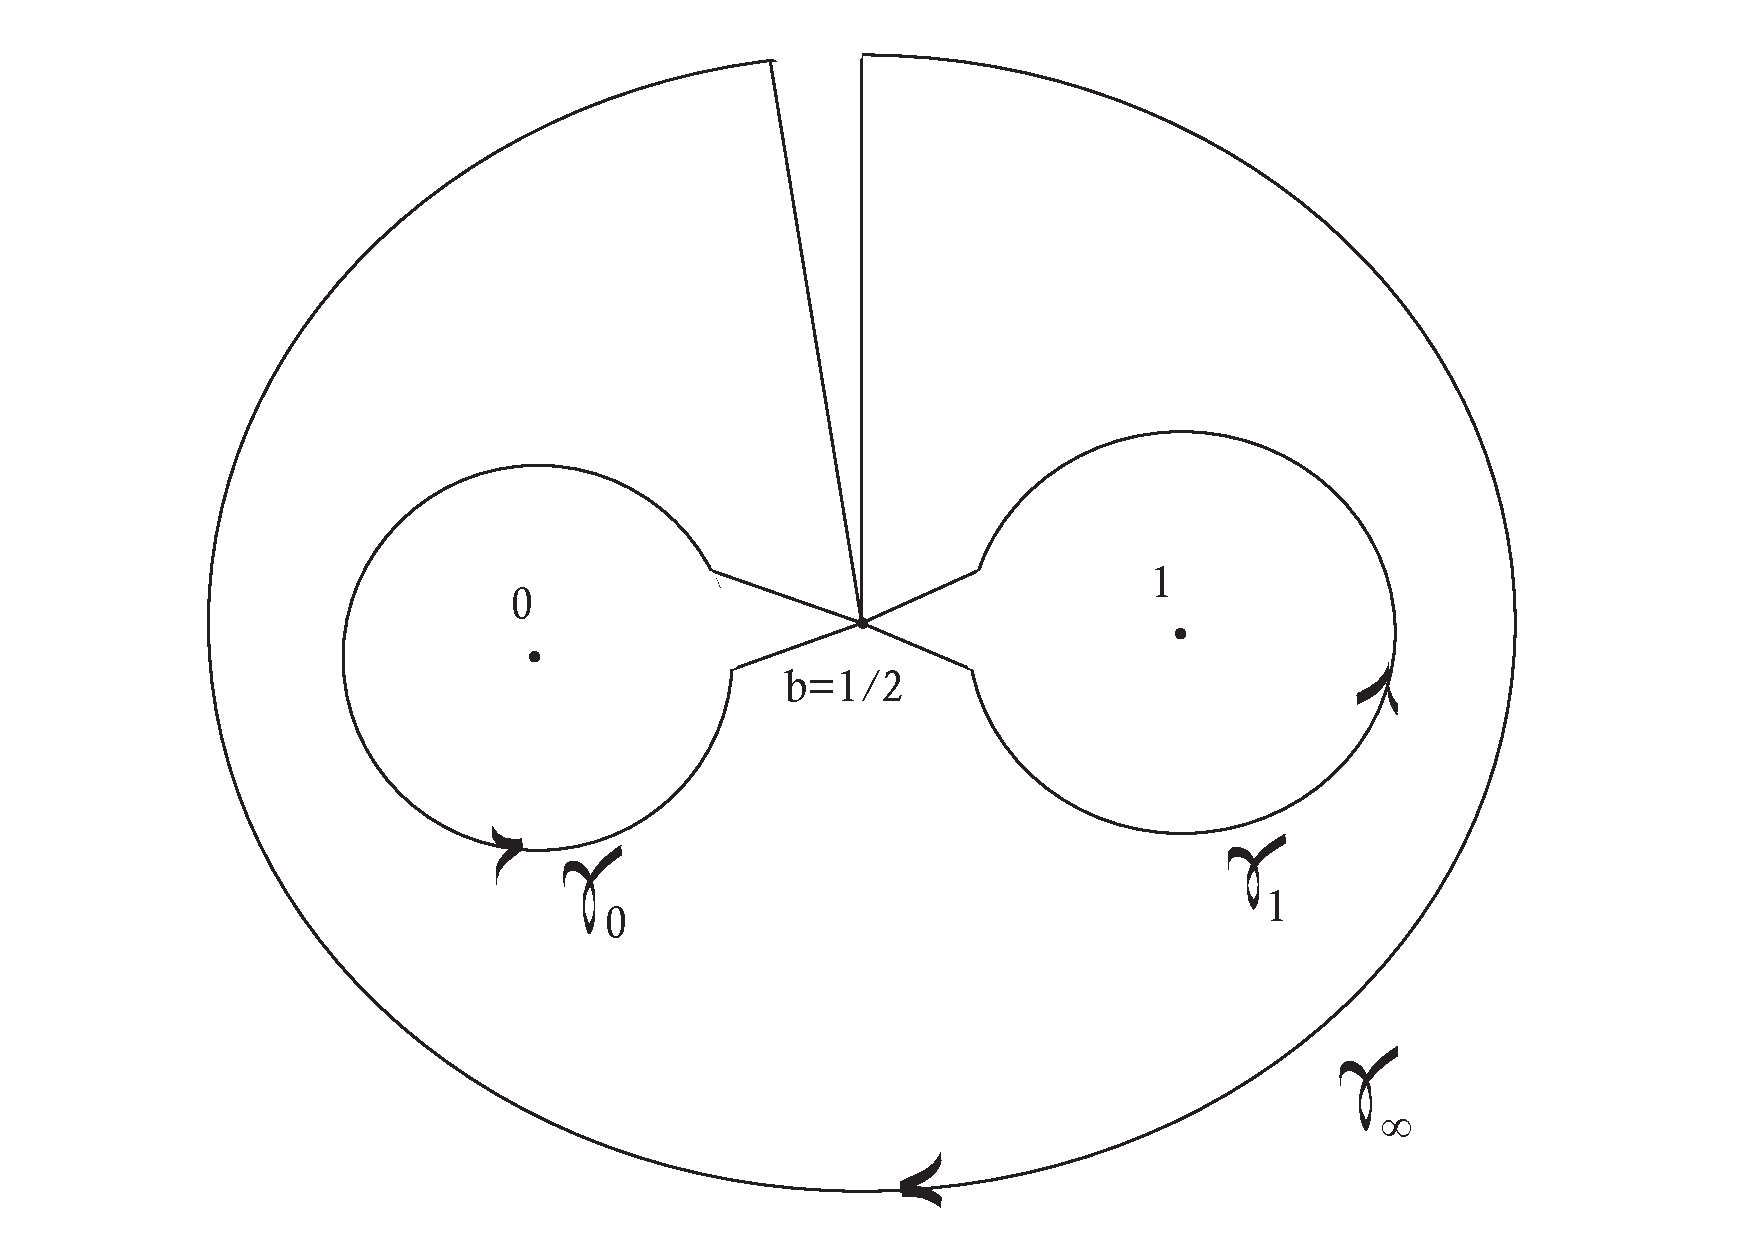
\includegraphics[width=10cm]{lazos3.pdf}
  \caption{Lazos anclados en $b=\frac{1}{2}$} \label{lazos3}
\end{figure}


El problema de hallar la monodrom\'ia respectiva a una ecuaci\'on diferencial es un problema complicado, afortunadamente existen m\'etodos que nos permiten hallar (en ciertos casos) la monodrom\'ia de la ecuaci\'on hipergeom\'etrica y tambi\'en el grupo de monodrom\'ia para soluciones particulares. En los siguientes cap\'itulos hallamos la monodrom\'ia de la ecuaci\'on hipergeom\'etrica y uno de los grupos de monodom\'ia respecto de las soluciones dadas en \ref{sec:sol_ec_hip}.


\section{Monodrom\'ia de la ecuaci\'on hipergeom\'etrica}

En esta secci\'on encontramos la monodrom\'ia de la ecuaci\'on hipergeom\'etrica a traves de su esquema de Riemann por medio de propiedades locales y la relaci\'on de Fuchs, utilizando fuertemente que la ecuaci\'on hipergeom\'etrica resulta ser irreducible.

Sea $G=\pi_{1} (D,b) $ y $\gamma_{j} \in G, (j=0,1,\infty )$, lazos en $b$. Sea $\rho: G \rightarrow GL(2,\mathbb{C}) $ una representaci\'on de monodrom\'ia del esquema de Riemann

\[ \left( \begin{array}{ccc}
0 & 1 & \infty \\
\rho_{1} & \sigma_{1} & \tau_{1} \\
\rho_{2} &\sigma_{2} & \tau_{2}  \end{array} \right)\]


Dado que 
\begin{equation}
\rho (\gamma_{1} \cdot \gamma_{0}) = \rho(\gamma_{\infty})^{-1}
\end{equation}

 ya que 
 \begin{equation}
 \gamma_{\infty}^{-1}=\gamma_{1} \gamma_{0}  y \gamma_{0}\gamma_{1}        
 \end{equation}
 
 
 es conjugado a $\gamma_{1} \gamma_{0}$, tenemos;

\begin{eqnarray} %equation
 \label{eqnarray:ecuacion1} \lbrace \varepsilon (\rho_{1}), \varepsilon (\rho_{2}) \rbrace \ conjunto \ de \ eigenvalores \ de \ \rho (\gamma_{0}) \\
 \lbrace \varepsilon (\sigma_{1}), \varepsilon (\sigma_{2}) \rbrace \  conjunto \ de \ eigenvalores \ de \ \rho (\sigma_{1}) \\
\lbrace \varepsilon(-\tau_{1}), \varepsilon (-\tau_{2}) \rbrace \  conjunto \ de \ eigenvalores \ de \ \rho (\sigma_{0} \sigma_{1})
\end{eqnarray}

Donde $\varepsilon (\cdot) = exp(2 \pi i \cdot)$. La clase de conjugaci\'on de $\rho$, es decir la monodrom\'ia de $RE(\rho,\sigma,\tau)$ esta casi determinada por los eigenvalores, y esta completamente determinada si la monodrom\'ia es irreducible.

\begin{defn}La ecuaci\'on de Riemann $RE(\rho,\sigma,\tau)$ se dice irreducible s\'i la monodrom\'ia es irreducible
\end{defn}

\begin{thm} \label{riemann-irreducible}

La ecuaci\'on de Riemann es irreducible si y solo si

$$\rho_{i} + \sigma_{j} + \tau_{k} \notin \mathbb{Z}, (i,j,k=1,2)  $$
Bajo esta condici\'on la representaci\'on $\rho $ se expresa hasta conjugaci\'on por las siguientes matrices:

$$ \rho (\gamma_{0}) \leftrightarrow  \begin{pmatrix}
 \varepsilon(\rho_{1})& 1\\
 0& \varepsilon(\rho_{2})
 \end{pmatrix}  ,\ \ \
\rho (\gamma_{1}) \leftrightarrow \begin{pmatrix}
 \varepsilon(\sigma_{1})& 0\\
 b& \varepsilon(\sigma_{2})
 \end{pmatrix}
$$

 Y el n\'umero $b$ esta dado por $b= \varepsilon(-\tau_{1}) + \varepsilon(-\tau_{2}) - \varepsilon(\rho_{1} + \sigma_{1}) - \varepsilon(\rho_{2} + \sigma_{2})$, y $\varepsilon(\cdot) =exp(2 \pi i \cdot)$. Todas las representaciones  obtenidas al intercambiar $\rho_{1},\rho_{2}$ y/o $\sigma_{1},\sigma_{2}$ son mutuamente conjugadas.

\end{thm}

En nuestro caso tenemos el esquema de Riemann;

\[ \left( \begin{array}{ccc}
0 & 1 & \infty \\
0 & 0 & a \\
1-c &c-a-b & b  \end{array} \right)\]

Y verificamos si satisface las condiciones del teorema, tenemos los siguientes casos:


\begin{enumerate}
\item 0+0+ a = a
\item 0 + c-a-b + b = c-a
\item 0 + c-a-b + a = c-b
\item 1-c + 0 + a= 1-c +a
\item 1-c + 0 + b=1-c+b
\item 1-c + c-a-b + b = 1-a
\item 0 + 0 + b = b
\item 1-c + c- a- b + a = 1-b
\end{enumerate}


 Queremos calcular $a,c-a,c-b,1-c+a,1-c+b,1-a,b,1-b$, y estamos considerando que los exponentes $ 1-c,c-a-b,a-b$ son imaginarios puros, por lo que basta probar que ninguno de los anteriores estan en $\mathbb{Z}$.

No es dif\'icil verificar que $b = \frac{1-i(\theta_{0} + \theta_{1} +\theta_{2})}{2} \notin \mathbb{R}$. Para $a$ tenemos;

$$a= \frac{1-i(\theta_{0} + \theta_{1} - \theta_{2})}{2}$$

Y podemos ver que $a \notin \mathbb{R}$ o $ a = \frac{1}{2}$  de cualquier modo $a \notin \mathbb{Z}$. Para $c-a$ se tiene;

$$c-a = \frac{1 + i (-\theta_{0} + \theta_{1} - \theta_{2})}{2}$$

Por lo que de nuevo $c-a \notin \mathbb{R}$ o $c-a = \frac{1}{2}$, y de cualquier modo $c-a \notin \mathbb{Z}$. Para $c-b$ se tiene;

$$c-b =\frac{1+i(\theta_{2} + \theta_{1} - \theta_{0})}{2} $$

Entonces $c-b \notin \mathbb{R}$ o $c-b =\frac{1}{2}$ y en cualquier caso $c-b \notin \mathbb{Z}$. Para $1-c+a$ notamos que $1-c+a= - (c-a-1 )$ y $c-a-1 = -\frac{1}{2}$ o $c-a-1 \notin \mathbb{R}$. En los casos restantes un proceso an\'alogo nos enseña que ninguno de los n\'umeros considerados esta en $\mathbb{Z}$.

Invocamos el teorema \ref{riemann-irreducible} al esquema de Riemann que hallamos para nuestra ecuaci\'on, y obtenemos que las matrices que generan la monodromia de la ecuaci\'on hipergeom\'etrica con exponentes imaginarios puros son:

$$ \rho (\gamma_{0}) \leftrightarrow  \begin{pmatrix}
 1& 1\\
 0& e^{2 \pi i (1-c)}
 \end{pmatrix}  ,\ \ \
\rho (\gamma_{1}) \leftrightarrow \begin{pmatrix}
 1& 0\\
 b& e^{2 \pi i (c-a-b)}
 \end{pmatrix}
$$

Con $b = e^{-2 \pi i a} + e^{-2 \pi i b} -1 -e^{2 \pi i (1-a-b)}$, y la monodrom\'ia de la ecuaci\'on hipergeom\'etrica es generada por $\rho (\gamma_{0}), \rho (\gamma_{1})$ en $GL(2, \mathbb{C})$.


\section{Grupo de monodrom\'ia con las soluciones dadas por la serie hipergeom\'etrica}

 En este cap\'itulo pretendemos dar a conocer el grupo de monodrom\'ia con el par de sistemas fundamentales de soluciones hallados en \ref{sec:sol_ec_hip}, utilizando las identidades de $Gauss-Kummer$. El enfoque principal en este cap\'itulo es exponer las herramientas necesarias para ese prop\'osito y los resultados principales que llevan a una expresi\'on del grupo de monodrom\'ia con los sistemas fundamentales de soluciones dadas. Los teoremas y resultados de este cap\'itulo pueden encontrarse en \cite{gausspainleve} as\'i como sus demostraciones, y se remite al lector a dicha bibliograf\'ia para un desarrollo m\'as profundo de lo expresado aqu\'i. \\


 Queremos resolver el problema de conexi\'on utilizando las identidades de $Gauss-Kummer$ y encontrar generadores para el grupo de monodrom\'ia de la ecuaci\'on diferencial hipergeom\'etrica con las soluciones dadas en \ref{sec:sol_ec_hip}. Los sitemas fundamentales de soluciones son $(f_{0}(x;0),f_{0}(x;1-c))$ y $(f_{1}(x;0),f_{1}(x;c-a-b))$ , queremos encontrar una relaci\'on entre estos sistemas.

 \begin{thm} Si ninguno de los exponentes $c$ o $c-a-b$ es un entero entonces

 $$ \label{relacion_sistemas_soluciones} (f_{0}(x;0),f_{0}(x;1-c))=(f_{1}(x;0),f_{1}(x;c-a-b))P$$

 Donde $P$ es la matriz definida por

$$ \label{matriz_conexion} P =  \begin{pmatrix}
 \frac{\Gamma(c) \Gamma (c-a-b)}{\Gamma(c-a) \Gamma(c-b)} & \frac{\Gamma(2-c) \Gamma (c-a-b)}{\Gamma(1-a) \Gamma(1-b)}\\
 \frac{\Gamma(c) \Gamma (c-a-b)}{\Gamma(a) \Gamma(b)} & \frac{\Gamma(2-c) \Gamma (c-a-b)}{\Gamma(a-c+1) \Gamma(b-c+1)}
 \end{pmatrix}
$$

Y $\Gamma$ es la funci\'on Gamma.
 \end{thm}

 En nuestro caso los exponentes $1-c$ y $c-a-b$ estan en $i\mathbb{R}$ por lo que $c$ y $c-a-b$ cumplen las condiciones del teorema. \\

 Los lazos en la fig. \ref{lazos3} nos sirven para hacer la continuaci\'on anal\'itica del sistema fundamental de soluciones $(f_{0}(x;0),f_{0}(x;1-c))$ y gracias al teorema anterior sabemos que tendremos una matriz conjugada bajo $P$ que ser\'a generador de nuestro grupo de monodrom\'ia.

 \begin{thm}
 Sea $\gamma_{v}, (v=0,1) $ lazos con punto inicial y final $b=\frac{1}{2}$ definidos en \ref{lazos3}, supongamos que ni $c$ ni $c-a-b$ son enteros. La continuaci\'on anal\'itica del sistema fundamental de soluciones $\mathfrak{F}=(f_{0}(x;0),f_{0}(x;1-c))$ a lo largo de $\gamma_{v}$ esta dada por

 $$\label{sistema_soluciones_continuacion_analitica} \gamma_{v_{*}} \mathfrak{F} = \mathfrak{F} A_{v} , (v=0,1)$$

 Donde $A_{v} $ son matrices definidas por

 $$ \label{Matrices_teorema_monodromia_grupo}  A_{0} =  \begin{pmatrix}
 1& 0\\
 0& \varepsilon (-c)
 \end{pmatrix}  ,\ \ \
A_{1} = P ^{-1}\begin{pmatrix}
 1& 0\\
 0& \varepsilon (c-a-b)
 \end{pmatrix} P
$$

Donde $P$ esta dada por \ref{matriz_conexion} y $\varepsilon(\cdot) = exp(2 \pi i \cdot )$. El grupo de monodrom\'ia respecto al sistema fundamental de soluciones $\mathfrak{F} $ esta generado por $A_{0}$ y $A_{1}$.
 \end{thm}

